\documentclass{article}
\usepackage{graphicx}
\usepackage{float}
\usepackage{caption}
\usepackage{subcaption}

   \graphicspath{{./images/}}

   \title{Final Report}
   \author{Team: AErenroc, SotoRivero, Zedbed}
   \date{December 5, 2025}


   \begin{document}
   \maketitle

   %\begin{abstract}
   %   Optional abstracte.
   %\end{abstract}

   \section{Introduction}
   % ~0.5 page
   Our project examines how politician Xi Jinping is presented to western audiences, with a focus on differences between North American and non–North American coverage.
   Our findings reveal a clear divergence in how Xi Jinping is framed across regions: North American outlets consistently emphasize negative themes such as human-rights
    issues, internal politics, and military policy. Whereas non-North-American sources offer more neutral or positive portrayals, especially in diplomatic and foreign 
    economic topics. We also find a temporal shift in sentiment/favorability on Xi Jinping in the media. 
   

   \section{Data} % - - - - - - - - - - - - - - - - - - - - - - - - - - - - - - - - - - - -
   % ~0.5 page
   We collected 502 English-language articles referencing Xi Jinping using TheNewsAPI, 
   drawn from 78 unique news sources. Articles were categorized by source region into: 
   

   \begin{itemize}
      \item North American: 287 articles
      \item Non-North American: 215 articles (including 8 European articles)
   \end{itemize}
   Because we restricted the dataset to English language only, 
   this clearly introduces potential biases. Non-NA articles written in English may 
   reflect more moderate or internationally ‘palatable’ positions for western audiences, 
   compared to articles in their own language. To make up for this somewhat we tried to include a wide 
   range of sources from differing regions, however there were still some news outlets that
   dominated publication frequency, as shown in Figure~\ref{fig:top_35_most_common_sources}.
   
   %\begin{figure}[H] % INSERTS IMAGE
   %     \centering
   %     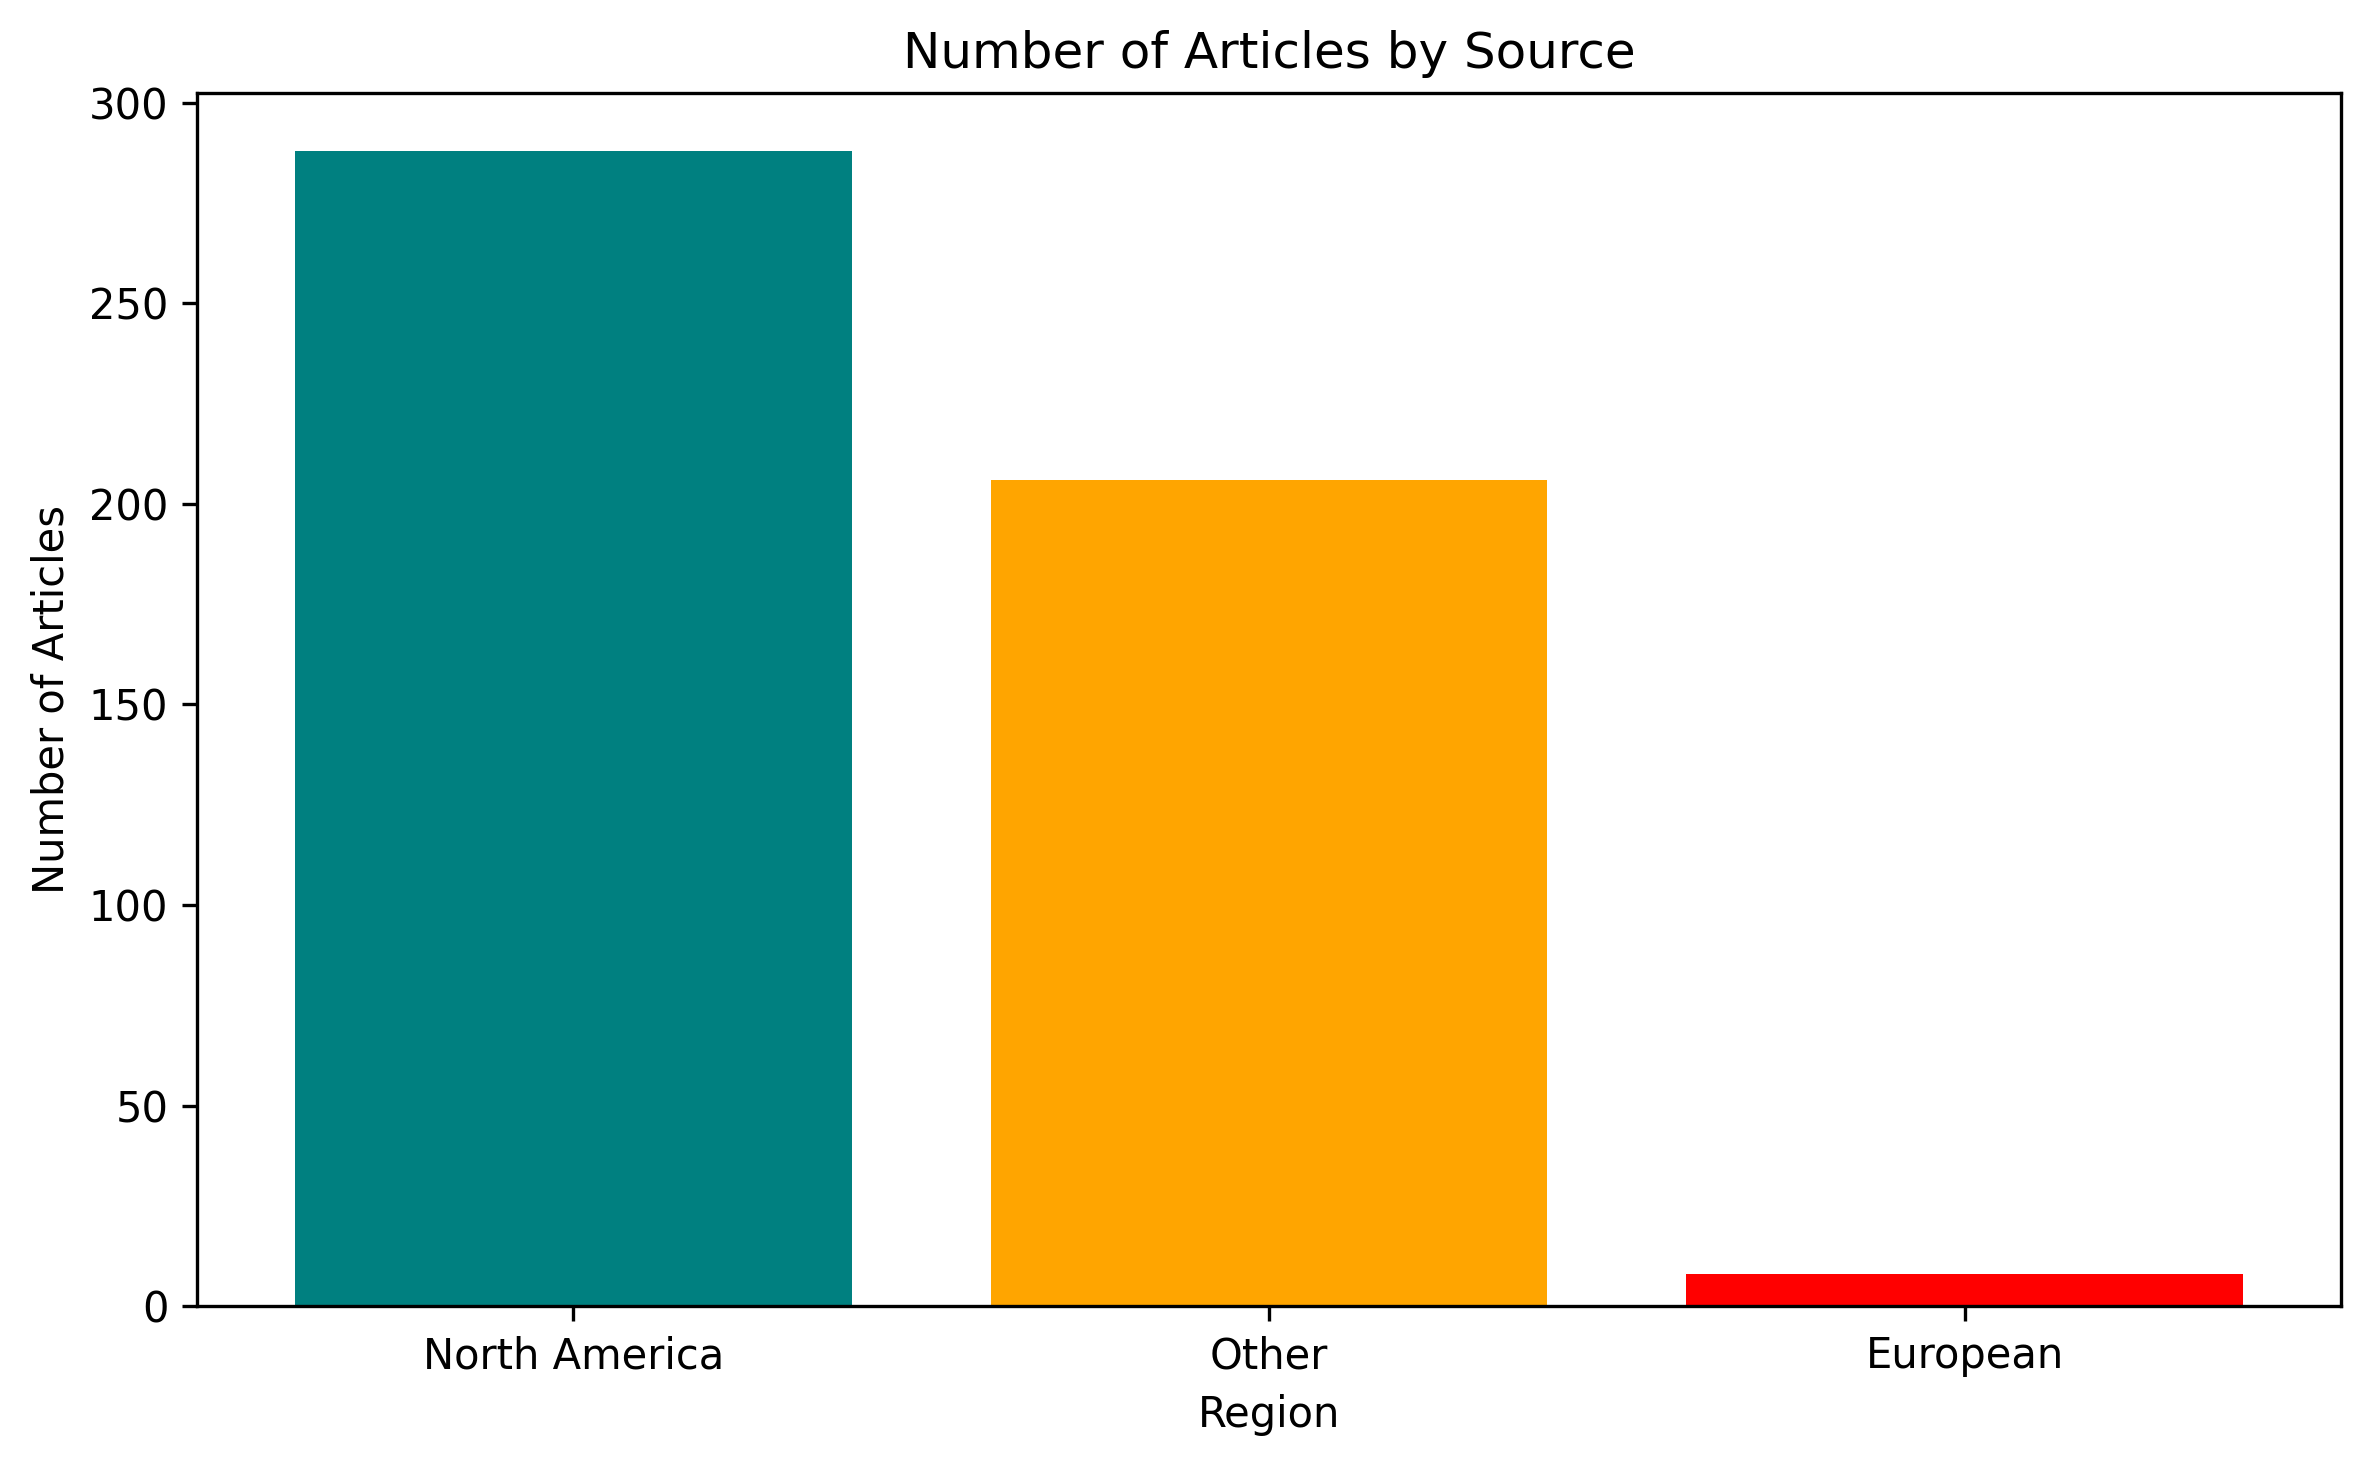
\includegraphics[width=0.5\textwidth]{num_articles_by_source_type.png} % or .png, .pdf, etc.
   %     \caption{Number of collected articles by source type.}
   %     \label{fig:articles_by_source_type}
   %\end{figure}

   \begin{figure}[H] % INSERTS IMAGE
        %\centering
        \hspace*{-2cm} % Moves the image over to the left
        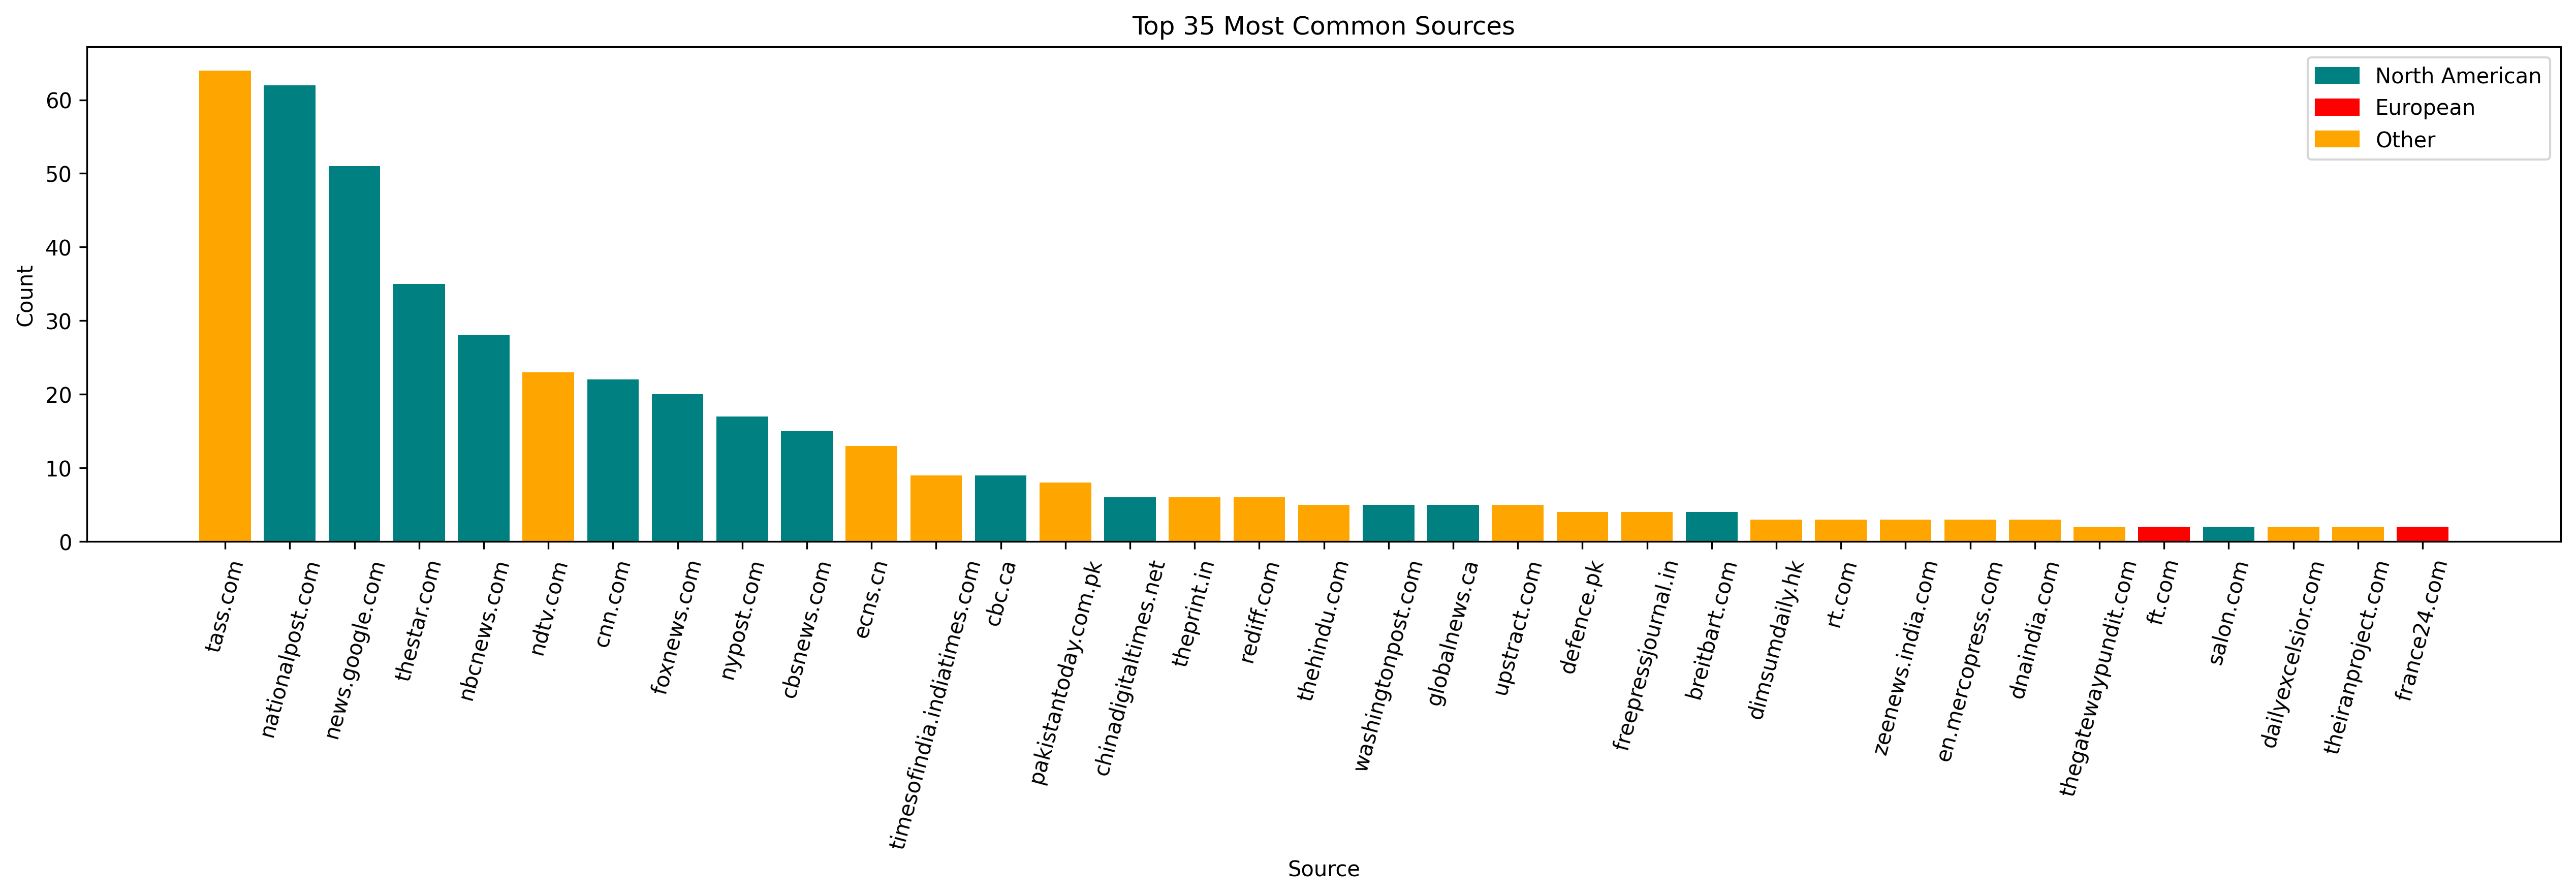
\includegraphics[width=1.3\textwidth]{top_35_most_common_sources.png} % or .png, .pdf, etc.
        \caption{The top 35 posters of articles on Xi Jinping.}
        \label{fig:top_35_most_common_sources}
   \end{figure}

   Future improvements to this project could include annotating non-English articles. 
   However, since our goal was to analyze how Xi Jinping is presented to western audiences, 
   the English language bias in our dataset is both expected and useful for this project analytically.



   \section{Methods} % - - - - - - - - - - - - - - - - - - - - - - - - - - - - - - - - - - - -
      % ~0.5 page
      We used human annotation combined with majority-vote aggregation for both the 
      labeling of topics articles cover and their respective sentiments to Xi Jinping.
      We also used tf-idf to explore the variation of topics North American vs Non-North American sources focused on.
      \\ \\
      The original project guidelines recommended analyzing 500 North American articles, however, open coding of an initial 
      North American sample showed very limited topic variation and predominantly negative sentiment, making it difficult to 
      identify more interesting or useful patterns. To address this, we decided upon a dataset of 287 North American and 215 
      non-North American articles, allowing for a more comparative analysis of how Xi Jinping is framed In comparison to other regions.

   
   \subsection{Typology}
      
      \begin{enumerate}
         \item \textbf{Domestic economic policy} - Economic growth, private sector regulation, modernization, development strategies.
         \item \textbf{Foreign economic policy} - Trade relations, tariffs, investment flows, global economic institutions.
         \item \textbf{Diplomatic relations} - Diplomatic events, summits, international negotiations.
         \item \textbf{Domestic social policy} - Civil liberties, minority groups, internal governance, surveillance, social stability.
         \item \textbf{Foreign social policy} - Cultural diplomacy, humanitarian engagements, public health, information policy.
         \item \textbf{Military policy} - Defense modernization, strategic posturing, security alliances.
         \item \textbf{Biographic} - Personal background, political career, leadership style.
         \item \textbf{Internal politics} - CCP leadership dynamics, party congresses, anti-corruption campaigns.
      \end{enumerate}
   Negative, Neutral and Positive sentiment was judged based on how each article framed Xi Jinping rather than the average perspective of a North American. For example, mentions of human rights violations by the article would frame Xi as ‘Negative’, whereas mentions of a flourishing economy under Xi would be ‘Positive’.


  
   \section{Results} % - - - - - - - - - - - - - - - - - - - - - - - - - - - - - - - - - - - -
   % ~1 page

   The first result we can observe is that our sample is pretty well balanced in terms of favourability.
   The selection of articles is pretty evenly split between Positive (25.5\%), Negative (36.1\%) and Neutral (38.4\%),
   coverage of Xi Jinping, with slighly more neutral and negative articles. 
   
   %\begin{figure}[H]
   %   \centering
   %   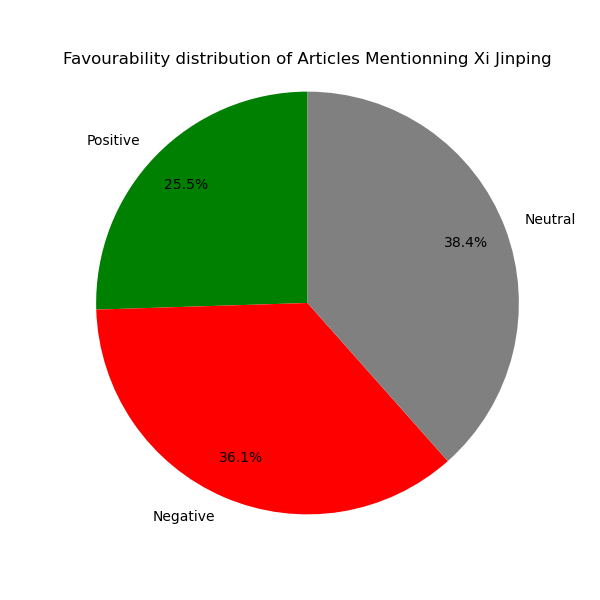
\includegraphics[width=0.45\linewidth]{pie_chart_Favourability_of_articles.png}
   %   \caption{Favorability distribution}
   %   \label{fig:pie_chart_Favourability_of_articles}
   %\end{figure}

   % Side-by-side figures
   \begin{figure}[H]
   \centering
   \begin{minipage}{.6\textwidth}
      %\centering
      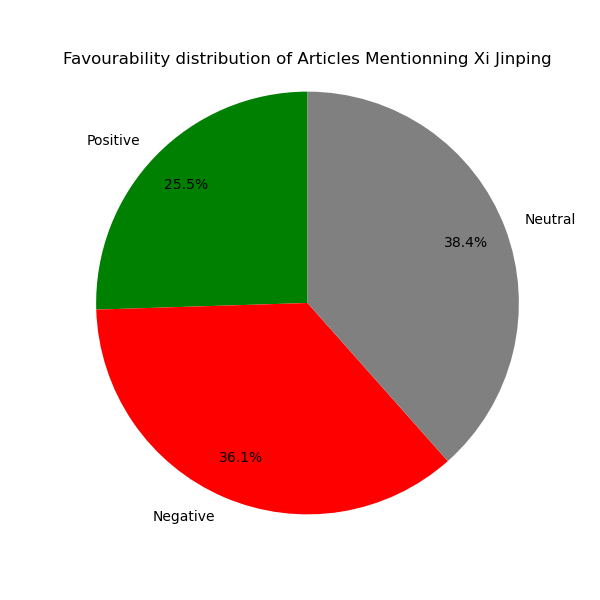
\includegraphics[width=.8\linewidth]{pie_chart_Favourability_of_articles.png}
      \captionof{figure}{Favorability distribution}
      \label{fig:pie_chart_Favourability_of_articles}
   \end{minipage}%
   \begin{minipage}{.6\textwidth}
      %\centering
      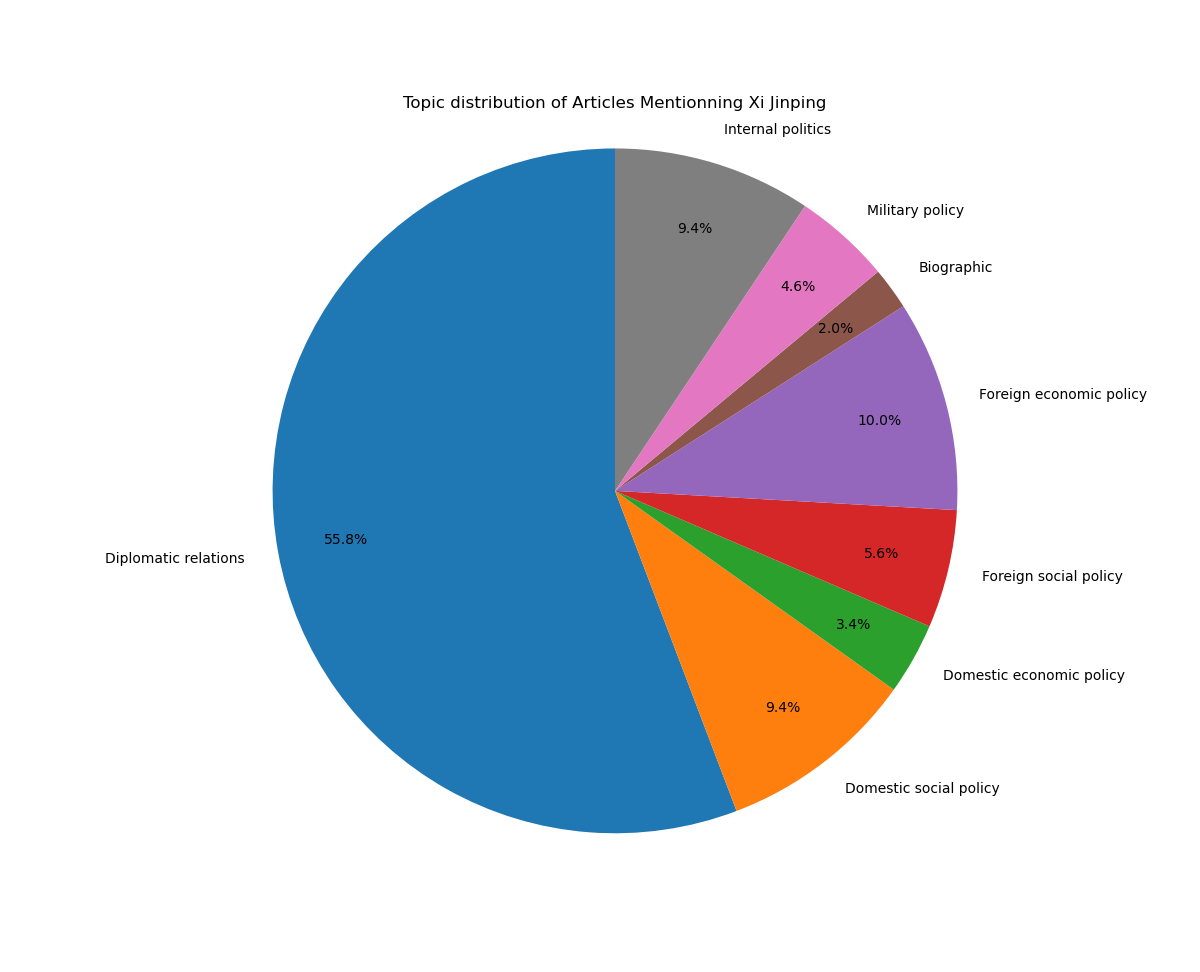
\includegraphics[width=1\linewidth]{Pie_chart_topic_distribution.png}
      \captionof{figure}{Topic distribution}
      \label{fig:Pie_chart_topic_distribution}
   \end{minipage}
   \end{figure}

   On the topic side, we observe that a majority (38.4\%) of articles have diplomatic relations 
   as their topic, with other significant topics being foreign economic policy (10.0\%), 
   internal politics (9.4\%) and domestic social policy (9.4\%). 
   This makes sense since a significant part of the coverage of Xi-Jinping in non-chinese media 
   consists of the mention of Xi's participation to various meetings and international events
   with ruler or official of their countries.   

   %\begin{figure}[H]
   %    \centering
   %    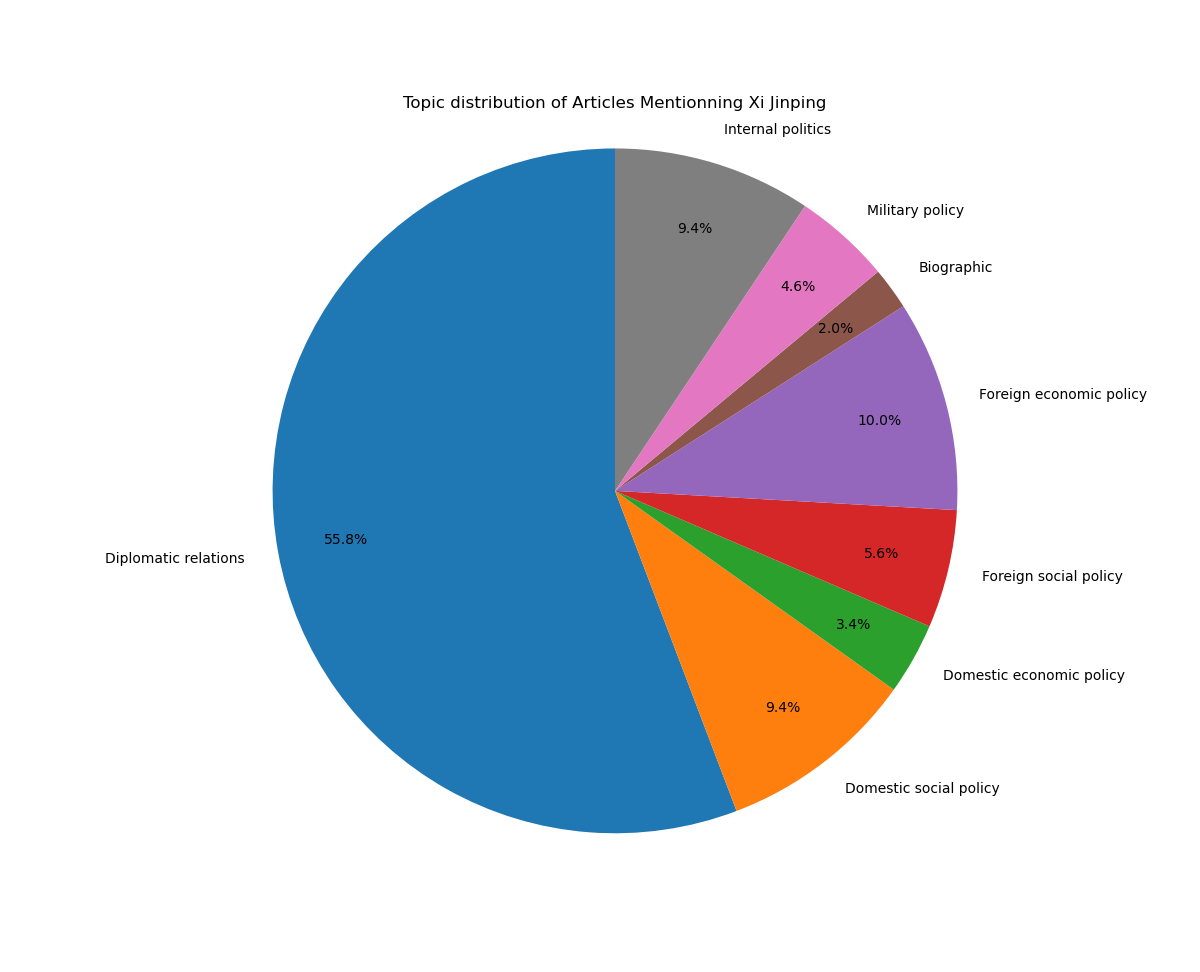
\includegraphics[width=0.65\linewidth]{Pie_chart_topic_distribution.png}
   %    \caption{Topic distribution}
   %    \label{fig:Pie_chart_topic_distribution}
   %\end{figure}

   Looking at the favourability of articles on these specific subject,
   we can see that articles about diplomatic relations are generally neutral 
   (45.7\%), or positive (28.9\%). This is also the case for Foreign economic 
   policy resp. (46.0\%) and (38.0\%). In contrast, articles about internal politics
   and domestic social policy are in majority negatives (68.1\%) and (61.7\%). 

   
   \begin{figure}[H] % INSERTS IMAGE
        \centering
        %\hspace*{-0.5cm} % Moves the image over to the left
        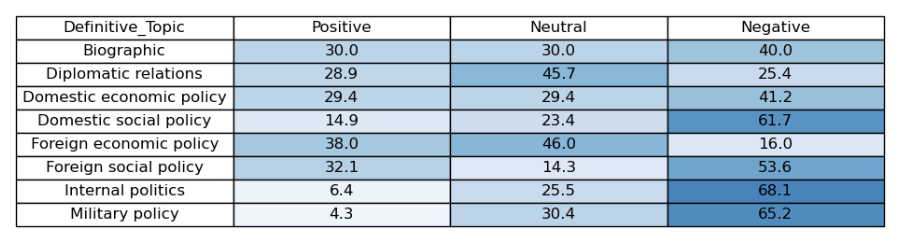
\includegraphics[width=0.8\textwidth]{croped_Favorability_per_topic_table.png} % or .png, .pdf, etc.
        \caption{Favorability of Articles per Topic}
        \label{fig:Favorability_per_topic_table}
   \end{figure}

   Looking now at the evolution of these metrics trough time, we can 
   see that the coverage of Xi-Jinping went from mostly negative or neutral in 2022 
   and 2023 to mostly positive in 2024. This can be explained by a lot of factors, which
   will be discussed more extensively in the findings section. 

   \begin{figure}[H]
      \centering
      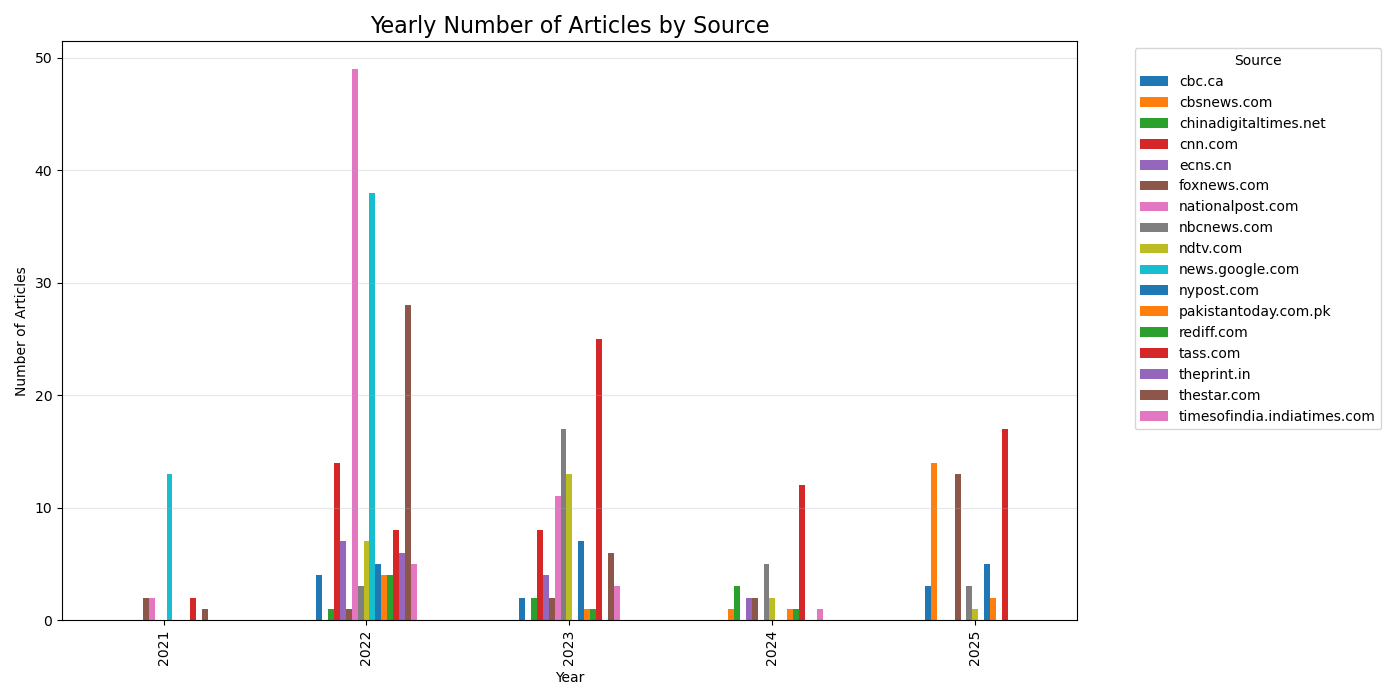
\includegraphics[width=0.8\linewidth]{images/Yearly_Articles_by_source.png}

      \label{fig:Yearly_Articles_by_source}
   \end{figure}


   It should also be noted that a big part of this change can probably be explained a shift in the mix of our sources between those years. As the most important sources for our articles went from the national post, google news and fox news in 2022 to tass being the most important in 2023 and onward.

   \begin{figure}[H]
      \centering
      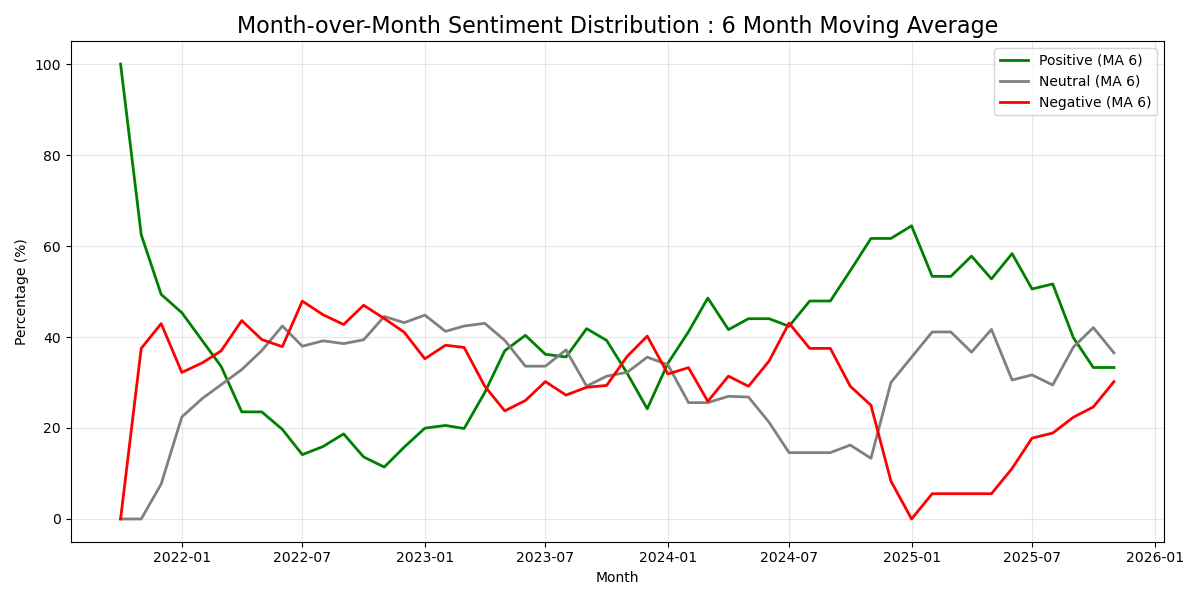
\includegraphics[width=0.8\linewidth]{images/6_month_mouving_average_favourability.png}

      \label{fig:6_month_mouving_average_favourability}
   \end{figure}

   This is notable since these sources seems to have different favourability levels for Xi Jinping, with tass articles in particular being generally positive (67.2\%).


   \begin{figure}[H] % INSERTS IMAGE
         %\centering
         \hspace*{-2cm} % Moves the image over to the left
         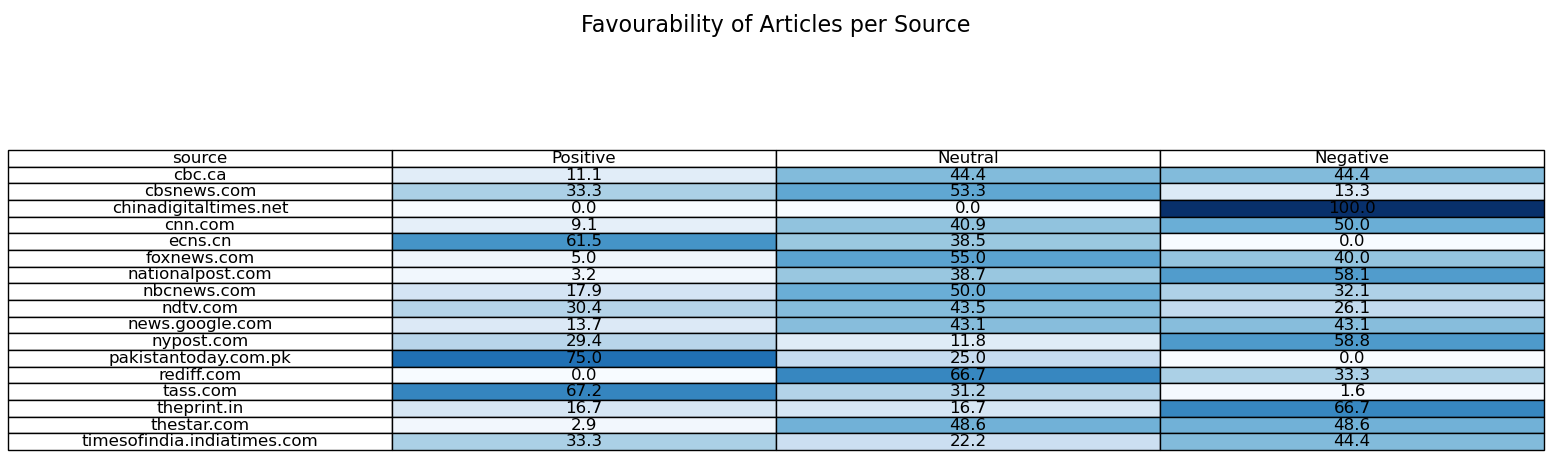
\includegraphics[width=1.3\textwidth]{images/Favourability_of_articles_per_source_table.png} % or .png, .pdf, etc.
      
         \label{fig:Favourability_of_articles_per_source_table}
      \end{figure}



   If we look specifically at North-American vs non North American sources, we can see that the North-American coverage stays and even becomes more negative, while the non North American coverage follows almost exactly the opposite pattern.


   \begin{figure}[H]
      \centering
      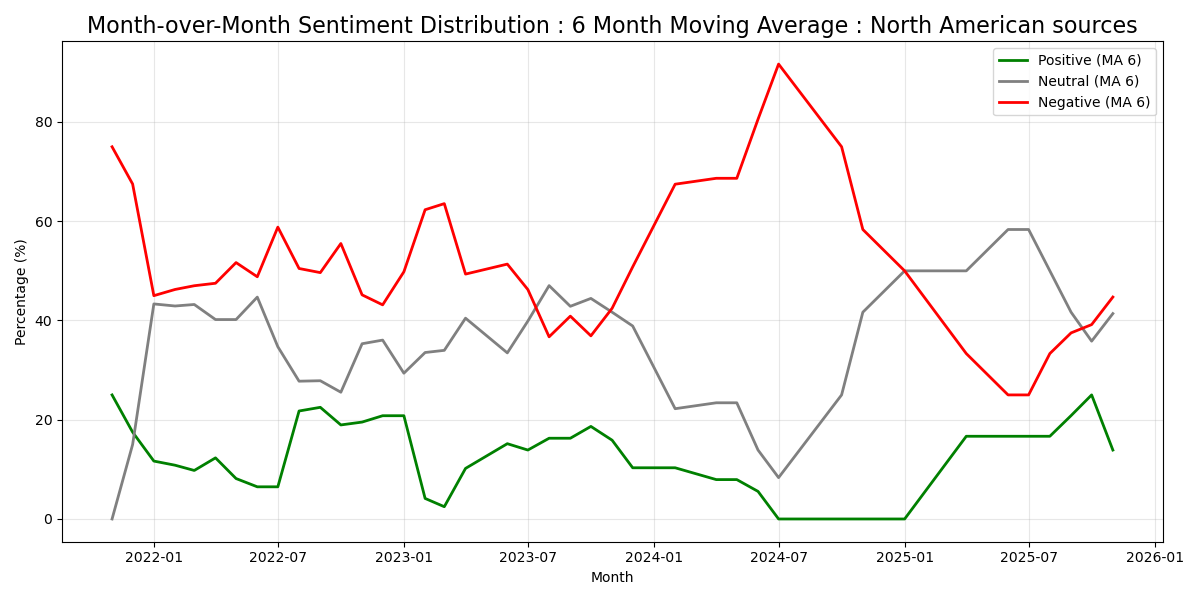
\includegraphics[width=0.8\textwidth]{images/6_month_mouving_average_favourability_NA.png}

      \label{fig:6_month_mouving_average_favourability_NA}
   \end{figure}

   \begin{figure}[H]
      \centering
      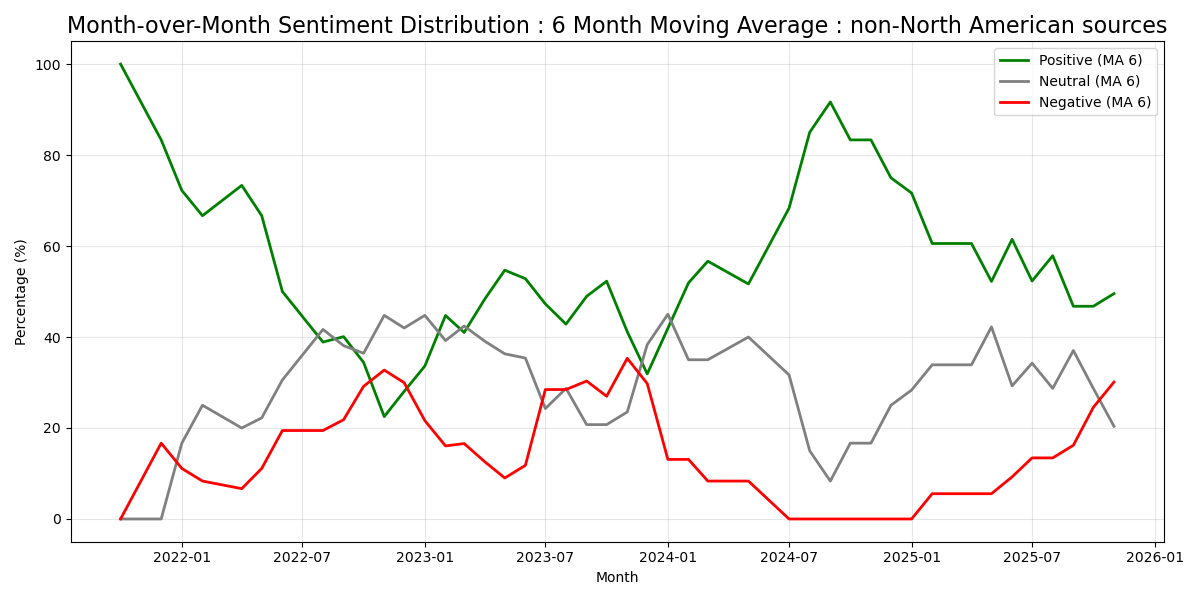
\includegraphics[width=0.8\linewidth]{images/6_month_mouving_average_favourability_non_NA.png}

      \label{fig:6_month_mouving_average_favourability_non_NA}
   \end{figure}











   \subsection{Regional Sentiment Patterns}
   Figures \ref{fig:aFavourability_NA_Sources} and \ref{fig:aFavourability_Other_Sources} illustrate sentiment distributions for North American and Non-NA sources:
   \begin{itemize}
      \item \textbf{NA:} Predominantly negative, especially on Domestic Social Policy, 
      Internal politics and Military policy. Issues of tariffs and domestic COVID19 policy are commonly covered.
      \item \textbf{Non-NA:} More neutral, with positive framing in Diplomatic Relations and 
      Foreign Economic Policy, especially when it comes to China's relations to non-western countries such as Russia.
   \end{itemize}


   % Side-by-side figures
   \begin{figure}[H]
   \centering
   \begin{minipage}{.6\textwidth}
      \centering
      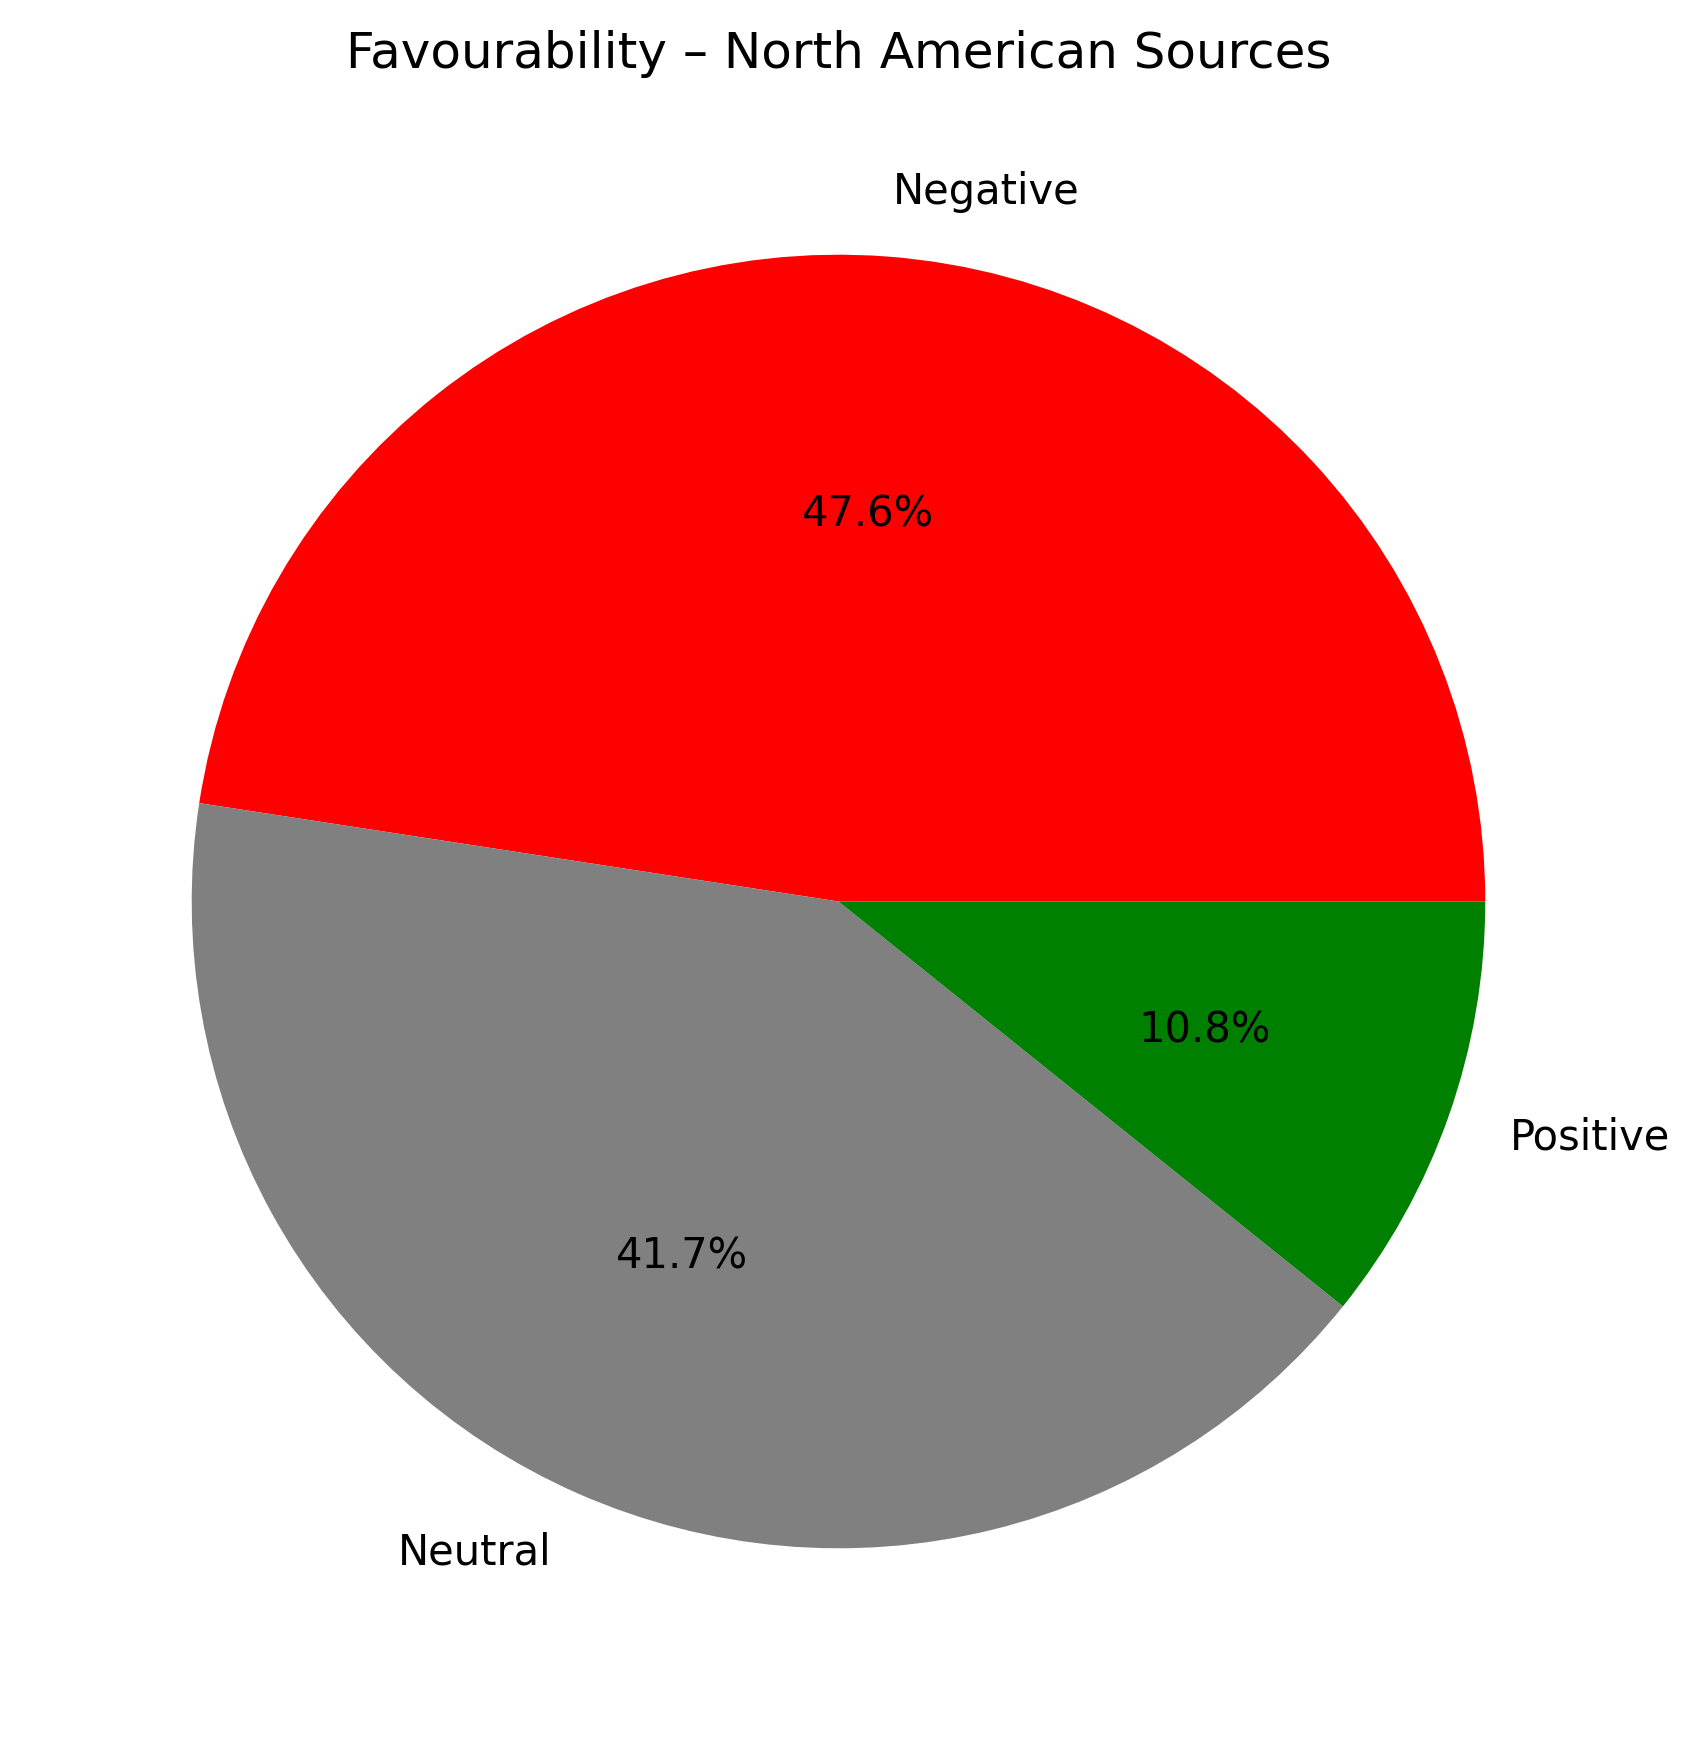
\includegraphics[width=.4\linewidth]{aFavourability_NA_Sources.png}
      \captionof{figure}{North American Favourability}
      \label{fig:aFavourability_NA_Sources}
   \end{minipage}%
   \begin{minipage}{.5\textwidth}
      \centering
      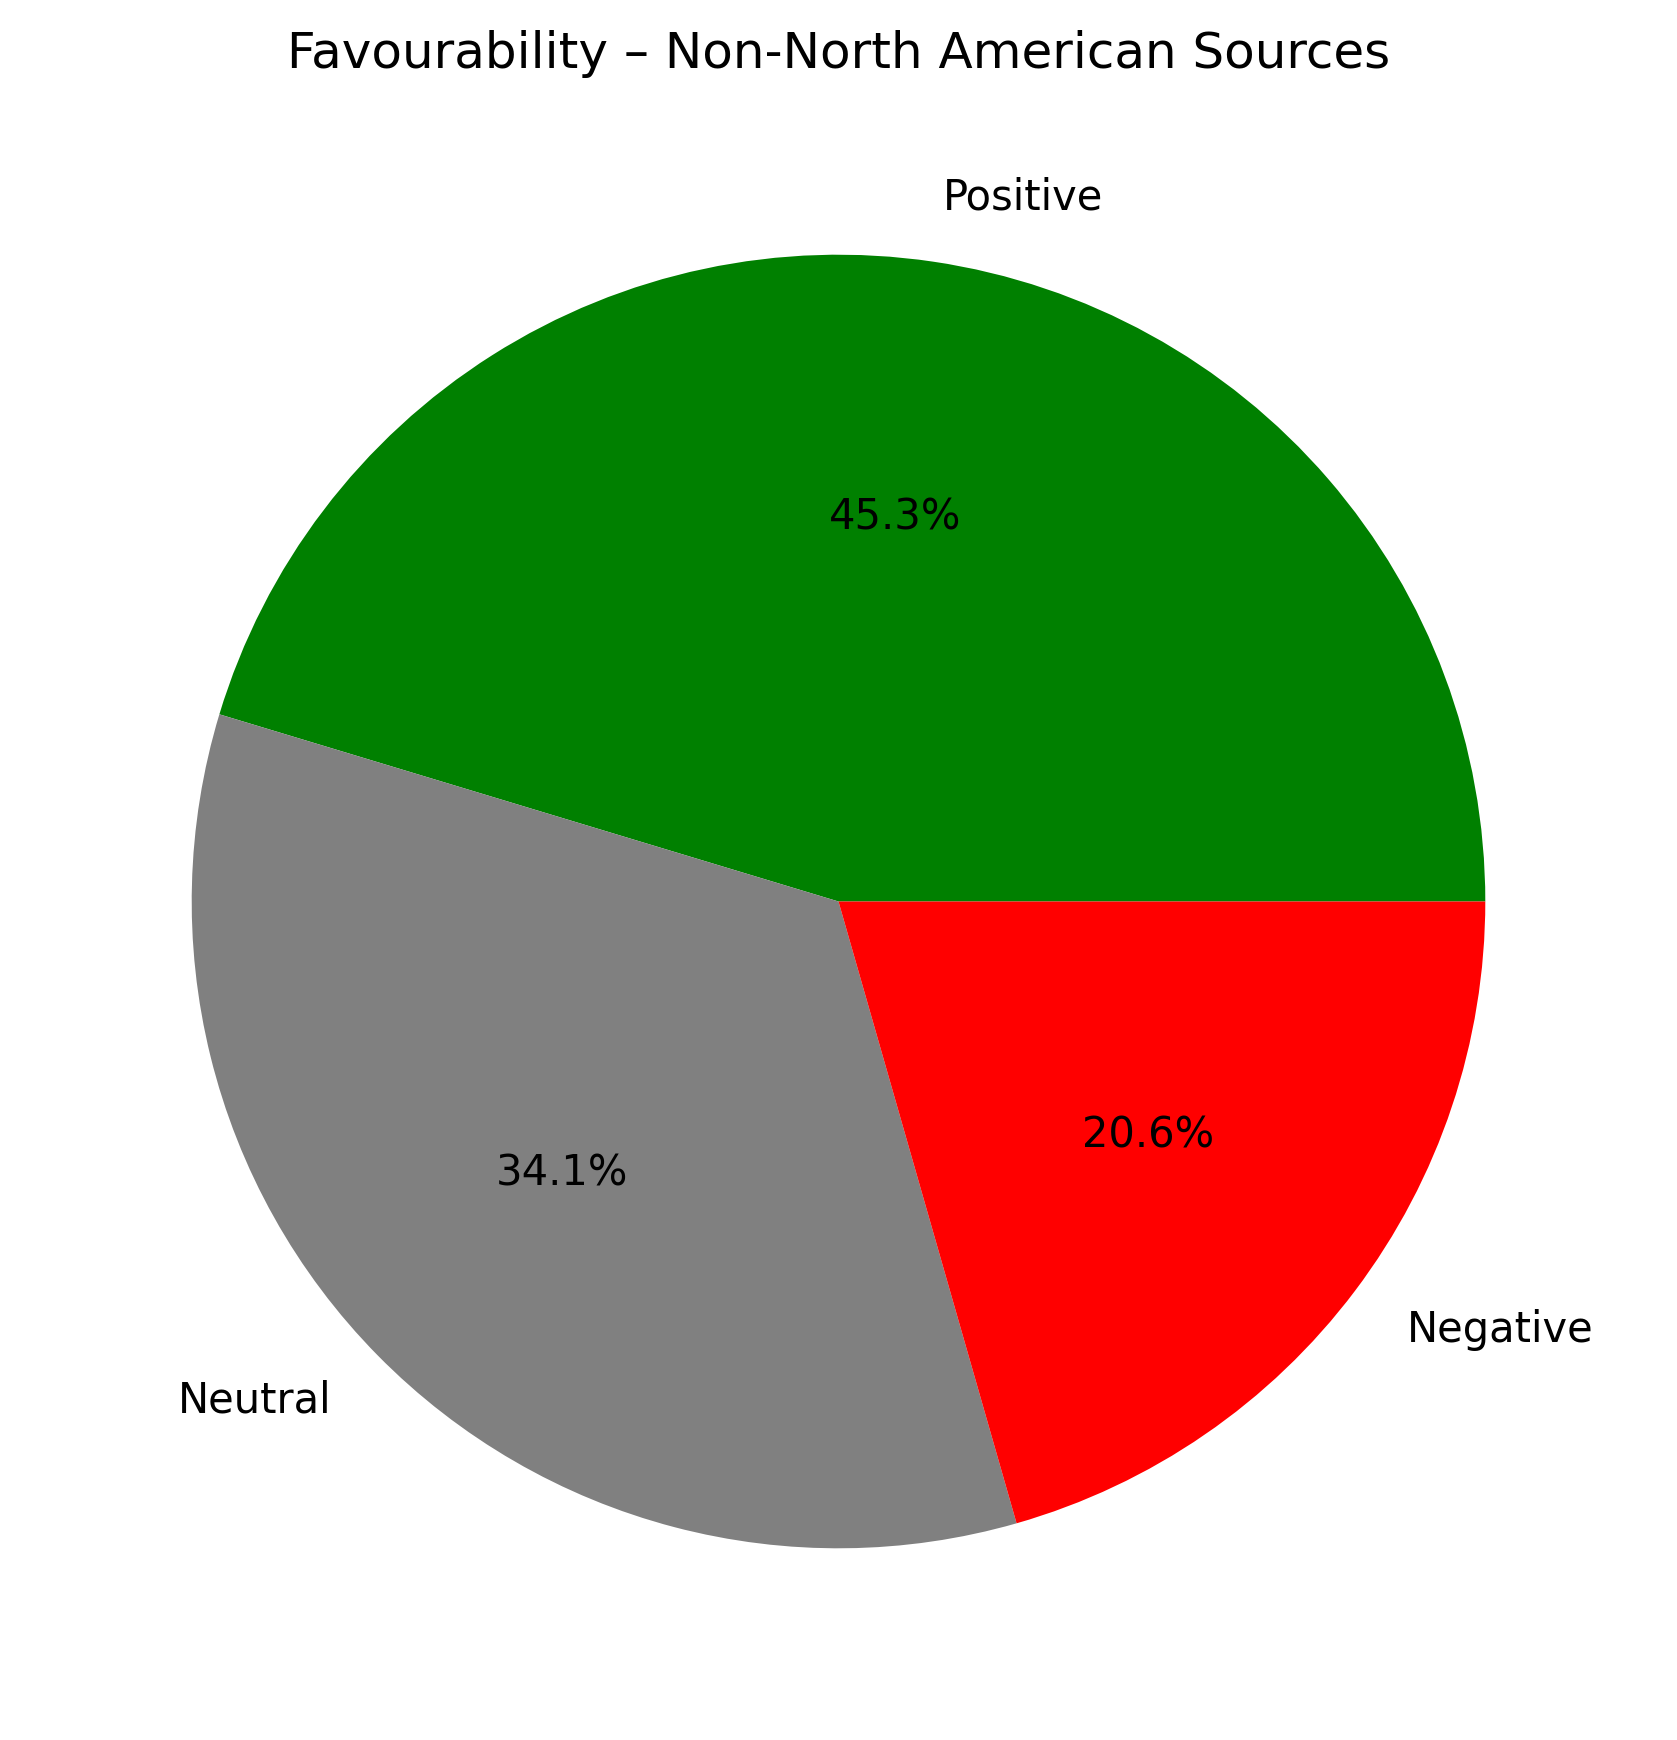
\includegraphics[width=.5\linewidth]{aFavourability_Other_Sources.png}
      \captionof{figure}{Other Source Favourability}
      \label{fig:aFavourability_Other_Sources}
   \end{minipage}
   \end{figure}


   
   





   \subsection{TF-IDF}
   %TOP 10 TERMS and their 10 HIGHEST tf-idf scored words: 
   %\\ \textbf{Domestic economic policy}:\\
   %-\hspace{0.5cm}\textit{NA}: terms such as “devastating,” “crisis,” and references to market instability. \\
   %-\hspace{0.5cm}\textit{Non-NA}: emphasizes “modernization,” “recovery,” “development,” and high-quality growth.
   %\\This indicates opposing framing: NA emphasizes risks, while Non-NA emphasizes progress.
   %\\ \textbf{Foreign economic policy}:\\NA sources:\hspace{0.5cm}(trade,trump,tariffs,deal,tariff,agreement,investment,tiktok,Bessent,BRICs)
   %\\ \textbf{Diplomatic relations}:\\NA sources:\hspace{0.5cm}(Putin,meet,Trudeau,Kremlin,friendship,diplomatic,Trump,minister,relations,northkorea)
   %\\ \textbf{Domestic social policy}:\\NA sources:\hspace{0.5cm}(Hong Kong,Uyghur,phase,unity,Xi,crackdown,fears,measures,Xinjiang,Muslims)
   %\\ \textbf{Foreign social policy}:\\NA sources:\hspace{0.5cm}(Putin,variant,Palestinian,xi,vladimir,Ukraine,skip,letup,bangladeshi,girl)

   \textbf{Domestic economic policy} \\
   NA: terms such as “devastating”, “crisis” and references to market instability.
   Non-NA: emphasizes “modernization”, “recovery”, “development” and "highquality".
   \\
      \textit{NA media emphasizes risk, while Non-NA emphasizes progress.}
   \\
   \textbf{Domestic social policy} \\
   NA: focuses heavily on “crackdowns”, “Uyghurs”, “Hong Kong”, “control”, focusing on minority rights.
   Non-NA: also some negative terms but with different emphasis e.g., “fears”, “collapse”, “COVID19.”
   \\
      \textit{Both regions portray this topic somewhat negatively, but NA discourse is more centered on human-rights.}
   \\
   \textbf{Foreign economic policy}
   \\
   NA: dominated by “Trump”, “tariffs”, "tiktok", “trade deals.”
   Non-NA: emphasizes positice relations such as “BRICS”, "cooperation" and "russia"
   \\
      \textit{Xi’s economic diplomacy is framed through U.S.–China conflict in NA, vs positive collaboration in Non-NA.}
   \\
      \textbf{Diplomatic relations}
   \\
   NA: uses terms like “Putin”, “Trudeau", "Trump", ”dictator" emphasizing geopolitical tension.
   Non-NA: more neutral presentation, including names like "Modi" and descriptors such as "summit" and "g20".
   




   \section{Findings} % - - - - - - - - - - - - - - - - - - - - - - - - - - - - - - - - - - - -
   % ~1 page
   Overall, we found that the north American and international coverage of Xi Jinping is somewhat balanced. 
   The majority of the coverage focus on international relation, but Foreign economic policy, Domestic social 
   policy and internal Chinese politics are also significant topics. There does not appear to be a significant 
   difference between the topic of North-American vs non-North-American sources. Over the whole 2022-2025, The 
   favourability as been pretty even between positive, negative and neutral coverage. Internal politics, 
   Military policy and Domestic social policy are the the subject on which ne coverage is the most negative, 
   often attacking Xi on the topics of respectively authoritarianism, the status of Taiwan and the treatement 
   of Uyghurs/state censorship. \\
    
    
   We can note an overall shift from a somewhat negative coverage to a somewhat positive coverage between the 
   end of 2023 and the first half of 2024. This may be due to different factors on the ground, including the end 
   of COVID restriction at the end of 2023 or an effort from China and its leaders to improve their image. The most 
   likely reason, however, seems to be a reduction in the frequency at which some (mostly critical) western outlets 
   mention the Chinese president, combined with an increase at which less critical non North-American sources mention 
   him. This could be due to Americans news outlets like Fox moving their focus away from international affairs to cover 
   the 2024 US presidential election. This can also highlight an increase in the importance of Russian-Chinese relations 
   after the 2022 invasion of Ukraine and subsequent sanctions, with a large number of articles from the Russian state 
   owned news agency Tass writing many positive articles about Xi. \\

   Overall, this shows a fracture in the way Xi Jinping is covered in North America vs the rest of the world. It also shows 
   how the reduced coverage of certain topics, like international affairs during a country's election, can shift the narrative
    by giving more place to non-traditional sources, like the Russian news agency tass.


   %notes -- China Russia relations are highly represented by non-north american sources and are positive to neutral, they focus on 
   %diplomatic relations more than domestic social policy or Military

   \section{Contributions} % - - - - - - - - - - - - - - - - - - - - - - - - - - - - - - - - - - - -
   \begin{itemize}
      \item \textbf{AErenroc}: Data collection, Code helpers/tools, Analysis, Report
      \item \textbf{Zedbed}: - Annotation, Analysis, Report
      \item \textbf{SotoRivero}: - Annotation, Analysis, Report
   \end{itemize}

   \end{document}